% Generated LaTeX file for compound CID: 12095
\documentclass[tikz]{standalone}
\definecolor{0000FF}{HTML}{0000FF}
\definecolor{274A4A}{HTML}{274A4A}
\definecolor{FF0000}{HTML}{FF0000}
\begin{document}
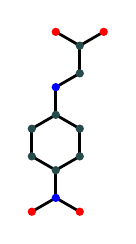
\begin{tikzpicture}[x=1pt,y=1pt]
  \draw[line width=1pt] (45.98,29.40) -- (37.32,24.40);
  \draw[line width=1pt] (28.66,29.40) -- (37.32,24.40);
  \draw[line width=1pt] (20.00,-35.60) -- (28.66,-30.60);
  \draw[line width=1pt] (37.32,-35.60) -- (28.66,-30.60);
  \draw[line width=1pt] (28.66,9.40) -- (28.66,-0.60);
  \draw[line width=1pt] (28.66,9.40) -- (37.32,14.40);
  \draw[line width=1pt] (28.66,-30.60) -- (28.66,-20.60);
  \draw[line width=1pt] (28.66,-0.60) -- (37.32,-5.60);
  \draw[line width=1pt] (28.66,-0.60) -- (20.00,-5.60);
  \draw[line width=1pt] (37.32,-5.60) -- (37.32,-15.60);
  \draw[line width=1pt] (20.00,-5.60) -- (20.00,-15.60);
  \draw[line width=1pt] (37.32,14.40) -- (37.32,24.40);
  \draw[line width=1pt] (28.66,-20.60) -- (37.32,-15.60);
  \draw[line width=1pt] (28.66,-20.60) -- (20.00,-15.60);
  \filldraw[fill=FF0000, draw=none] (45.98,29.40) circle (1.5pt);
  \filldraw[fill=FF0000, draw=none] (28.66,29.40) circle (1.5pt);
  \filldraw[fill=FF0000, draw=none] (20.00,-35.60) circle (1.5pt);
  \filldraw[fill=FF0000, draw=none] (37.32,-35.60) circle (1.5pt);
  \filldraw[fill=0000FF, draw=none] (28.66,9.40) circle (1.5pt);
  \filldraw[fill=0000FF, draw=none] (28.66,-30.60) circle (1.5pt);
  \filldraw[fill=274A4A, draw=none] (28.66,-0.60) circle (1.5pt);
  \filldraw[fill=274A4A, draw=none] (37.32,-5.60) circle (1.5pt);
  \filldraw[fill=274A4A, draw=none] (20.00,-5.60) circle (1.5pt);
  \filldraw[fill=274A4A, draw=none] (37.32,14.40) circle (1.5pt);
  \filldraw[fill=274A4A, draw=none] (28.66,-20.60) circle (1.5pt);
  \filldraw[fill=274A4A, draw=none] (37.32,-15.60) circle (1.5pt);
  \filldraw[fill=274A4A, draw=none] (20.00,-15.60) circle (1.5pt);
  \filldraw[fill=274A4A, draw=none] (37.32,24.40) circle (1.5pt);
\end{tikzpicture}
\end{document}